\documentclass[12pt, letterpaper]{article}
\usepackage[utf8]{inputenc}

\usepackage{geometry}
\geometry{
a4paper,
left=25mm,
right=25mm,
top=25mm,
bottom=25mm
}

\usepackage{multicol}

\usepackage{graphicx}
\graphicspath{ {images/} }
\usepackage{wrapfig}

\usepackage{textcomp}

\usepackage{hyperref}
\usepackage[all]{hypcap}

% Set the link style for the document.
\hypersetup{
colorlinks,
citecolor=blue,
filecolor=blue,
linkcolor=blue,
urlcolor=blue
}

\usepackage[explicit]{titlesec}

\titleformat{\paragraph}[runin]
{\normalfont\normalsize\bfseries}{\theparagraph}{1em}{#1\quad--}


% Start fix titlesec numbering.
\usepackage{etoolbox}
\makeatletter
\patchcmd{\ttlh@hang}{\parindent\z@}{\parindent\z@\leavevmode}{}{}
\patchcmd{\ttlh@hang}{\noindent}{}{}{}
\makeatother
% End fix titlesec numbering.


\providecommand{\keywords}[1]{\textbf{\textit{Keywords---}} #1}

% ==============================================================================



\title{Spectrangle}
\author{Wybe Westra --- s1578472}
\date{Software Systems \\ \today}

\begin{document}

    \maketitle

    \newpage

    \tableofcontents

    \newpage


    \section{Design}

    Spectrangle is implemented using a separate server and client.
    The game functionality is divided between the two according to the requirements laid out in the module manual,
    with one small exception.
    One cannot select a port for the server or client.
    This is because the network protocol determines that only port 4000 is to be used.

    Other than that, all the functionality required for single-person ``groups'' is implemented.

    % ------------------------------------------------------------------------------------------------------------------

    \subsection{Client and MVC}
    \label{subsec:clientAndMVC}

    \begin{figure}[ht]
        \begin{center}
            \includegraphics[width=\textwidth]{Client.png}
            \caption{Diagram depicting how the client functions.
            Red blocks are separate threads.}
            \label{fig:clientDiagram}
        \end{center}
    \end{figure}

    The client is designed using the Model-View-Controller pattern.
    As visible in~\autoref{fig:clientDiagram}, the classes are named according to their role.
    The ClientController fulfills the Controller role, the GameModel is the model,
    and the TuiView is a view that uses the terminal to communicate with the user.

    The GameModel only exists when there is a game ongoing.
    Outside of a game, the GameModel reference points to `null`.

    Also laid out in~\autoref{fig:clientDiagram} are the two threads that the client uses during runtime.
    The Network thread is responsible for receiving and parsing the messages received from the server.
    When a valid message is received, it calls the appropriate method on the ClientController.
    The controller then either updates the model, or directly calls a method on the view.
    The only times the controller directly calls the view, is outside of a game or when a chat message arrives.
    The chat message bypasses the GameModel because it is not really part of the game.

    The input thread is continuously reading from the TUI .
    The main reason it is done like this, instead of polling the user when input is needed, is to facilitate the chat
    mechanism.
    The program has no idea when the user might want to send a chat message, so it needs to continuously read the input.
    Doing this, and listening to the server at the same time necessitates two threads.
    It has the nice side-effect that it allows the user to also input other commands at any time.
    For example, one could input `exit` while being asked for what tile to place, and it would parse just fine.
    After the input thread parses the command, the appropriate method on the controller is called.

    The only state held by the view is the current prompt for the user, and the chat history.
    The rest of the state, including things like which move the user wants to make, is kept in the GameModel.

    The GameModel is implemented as an observable, and is observed by the view.
    When the GameModel is updated by the network thread, or the input thread, it notify's the observers, which in this
    case is only the view.
    The notification includes a reference to the GameModel itself, along with a GameModel.Change enum, that signals
    what kind of update this is.
    The view takes this update, and changes it's prompt to the user according to the current state of the GameModel.
    For example, if the GameModel notifies the view that the player should select a tile to place, the view will
    update it's prompt to reflect that.

    The GameModel contains several self-defined classes, some of which are shared with the server.
    A diagram of the GameModel and the classes it contains as fields, can be seen in~\autoref{fig:modelDiagram}.
    The functionality and storage formats used by these classes
    will be further elaborated in~\autoref{subsec:Descriptions}.

    % ------------------------------------------------------------------------------------------------------------------

    \subsection{Server}
    \label{subsec:serverDesign}

    \begin{figure}[ht]
        \begin{center}
            \includegraphics[width=\textwidth]{Server.png}
            \caption{Diagram depicting how the server functions.
            Red blocks are separate threads.}
            \label{fig:serverDiagram}
        \end{center}
    \end{figure}

    The server utilizes significantly more threads as the client.
    This can be seen in~\autoref{fig:serverDiagram}, where each red block represents a separate thread.

    The first thread to start is the main thread, which then starts up the Lobby thread.
    The main thread monitors the server socket, and creates a new ClientPeer for every connecting client.
    It starts the client's thread and then hands of the client to the Lobby, via a synchronized variable.

    Each ClientPeer thread continuously listens for messages from it's client.
    It parses each message, and if necessary sets a variable that indicates the client wants to do something.
    For example, each client has a queue of chat messages that it received.
    The thread currently responsible for that client periodically empties the queue and passes them on.
    The thread that has the client can also send messages through this connection, either by sending a raw string
    or via methods that implement messages from the networking protocol.
    Each client prints out the messages that get sent or received, so that it is clear what is going on.

    The Lobby receives new clients from the main thread and puts them in the waiting list.
    It periodically checks on the clients in this list, to see if they have requested a game, or if they have
    sent a chat message.
    There is a separate lobby list for each possible amount of players in a game, so 2, 3 and 4.
    The clients are placed in these lists after they have requested a game with the corresponding amount of players.
    Each list of players can only chat with the players in that list.

    After there are enough players, the Lobby starts a new Game.
    Each Game runs in a separate thread, so that two games won't step on each others toes
    and have to wait for each other.
    The Game enforces the rules, and keeps track of the tile bag, the Board, turn order, scores and other game
    related things.
    Details on how these are stored can be found in~\autoref{subsec:Descriptions}
    When a game finishes, the Lobby takes back the clients and puts them back into the waiting list.

    % ------------------------------------------------------------------------------------------------------------------

    \subsection{Class descriptions}
    \label{subsec:Descriptions}

    % ------------------------------------------------------------------------------------------------------------------

    \subsubsection{Game pieces}

    All the shared classes that are related to a game of Spectrangle.

    \paragraph{Abstract: AbstractPlayer}
    This abstract class is inherited by both the client's and the server's Player class.
    It keeps a list of all the Tiles a player has in their hand, along with the player's name
    and their current score.
    It also provides a method to subtract all the remaining tiles from the player's score, which get's used at the end
    of a Game.

    \paragraph{Board}
    Represents the triangular game board used in Spectrangle.
    It's built around an array of 36 BoardSpaces, which it instantiates with the bonus values as described in the rules.

    It provides methods to check whether a given Move is valid, as well as a method which actually makes the move
    and calculates the score of the move.
    There is also a method which will determine whether a given hand of Tiles would allow a player to make a move,
    which is used by the server in determining whether a player needs to skip or not.

    \paragraph{BoardCoordinates}
    A container of a column and a row number, that represent a specific space on the Board.
    Its purpose is to calculate which board spaces are next to each other, as this is almost
    impossible using only an index.

    This can be converted to and from a board index, and provides methods that return the coordinates of
    the requested neighbouring space.
    It is only used by the Board, for the purpose of these neighbour calculations.

    \paragraph{BoardSpace}
    Represents a spot on the game Board.
    This is used to store whether this space is a bonus space, along with the Tile that is on it.

    \paragraph{Move}
    Represents a move that can be made on a Spectrangle Board.
    Basically a wrapper around a Tile and a number that specifies a board index.
    This is a lot easier to pass around than two separate objects.

    \paragraph{Tile}
    A representation of the triangular tiles used in the game.
    It has three Colors, one for the `flat' side, one for the side clockwise of that, and one for the remaining side.

    Encoding it in this way allows one to check if two tiles are valid next to each other by checking the same side,
    so instead of having to check the `left' side of tile 1 and the `right' side of tile 2, one can simply check
    the `clockwise` side of both.

    Provides two methods for turning the tile, 120 degrees or 240 degrees, that return a new tile that is rotated
    the specified amount.
    The equals method checks for equality and equal same orientation.
    The isEquivalent method will regard rotated tiles as being equivalent.
    It also provides methods to convert to and from the string representation specified in the network protocol.

    \paragraph{Enum: Color}
    This enum encodes the colors that a side of a tile can have.
    Provides a method to check whether two colors are valid when placed next to each other.
    It has methods to convert a Color to and from the letters used in the network protocol.

    \paragraph{Interface: TileBag}
    Interface that specifies the possible interactions with a bag of Tiles.
    This is implemented by the RandomTileBag, as well as the MockTileBag that is used during testing.
    Ease of testing is also immediately why this interface exists, as a Game class that only accepts random
    tile bags is really hard to test in a deterministic way.

    \paragraph{RandomTileBag}
    This class implements the TileBag interface.
    Represents the bag of Tiles that is used in a Spectrangle game.

    It includes a method that fills the bag with all the starting Tiles as described in the rules of the game.
    It's implementation of the takeTile method returns a random Tile from the bag.

    \paragraph{EmptyTileBagException}
    This exception get's thrown by a TileBag when takeTile is called when the bag is empty.

    \paragraph{IndexException}
    This get's thrown by methods of Board and BoardCoordinates, either when a method is called with invalid
    coordinates, or when a method that returns coordinates can't return valid ones.

    \paragraph{InvalidMoveException}
    Thrown by the Boards makeMove method when the move is not a valid one.

    \paragraph{NoTileException}
    Thrown by the Boards getTile method when the space at the given id does not have a tile.

    % ------------------------------------------------------------------------------------------------------------------

    \subsubsection{Networking}

    All the shared classes related to the network communication.
    Both the client and the server have their own implementation of the AbstactPeer.

    \paragraph{Abstract: AbstractPeer}
    This abstract class is inherited by the ClientPeer and the ServerPeer.
    It provides common functionality needed by both sides of the network protocol.

    Keeps track of the Connection to the server or client, and implements the Runnable interface.
    Passing the class to a Thread will have that thread listen for messages comming in via the connection.
    When a message is received, the abstract method handleReceivedMessage is called.
    This method is implemented by the ClientPeer and ServerPeer, to provide the needed message parsing functionality.

    Also provides a method to send messages over the Connection, as well as a ``verbose'' option, which will make it
    print out every message that get's sent through it.
    The verbose option is used by the server, but not by the client.

    This class includes JML specifications.

    \paragraph{Interface: Connection}
    Interface that represents the ways in which the ServerPeer and ClientPeer classes can interact with a connection to
    another program.
    Is implemented by the SocketConnection, as well as the MockConnection, which is the test variant.

    Provides methods read messages from the connection, as well as send messages.
    Also provides a method to check if the connection is still alive, as well as a method to
    cleanly kill the connection.

    This interface is used instead of immediately calling methods of SocketConnection, to make it possible to use
    a non-internet version of the connection for unit testing purposes.

    \paragraph{SocketConnection}
    Implements the Connection interface.
    On construction it takes a connected Socket, which it uses to send and receive messages.
    It monitors the underlying socket, and when the socket closed the function isDead will return true.


    \paragraph{DeadConnectionException}
    Thrown by Connections when a readMessage or sendMessage is attempted, and the underlying connection is broken.

    \paragraph{DecodeException}
    Thrown by Color and Tile when the message passed to their decode methods fails to parse.

    \paragraph{InvalidCommandException}
    Thrown by the message parsing methods of the ServerPeer and ClientPeer classes.
    Indicates that the message given does not translate to a valid command.

    Usually leads to this error being printed, and an `invalidCommand' message being sent over the Connection.


    % ------------------------------------------------------------------------------------------------------------------

    \subsubsection{Client classes}

    These classes are exclusive to the client.

    \paragraph{Client}
    The main starting method of the client.
    The main method first asks which server address the user wants to connect with.
    Once the connection is established, it asks the user for a name, which it verifies with the server.
    When the name is valid it creates a ClientController with the created Connection and Name, it also passes along
    whether the server supports the chat extension or not.

    It then has the controller start it's View thread, and calls the run method of the ServerPeer.
    When the run method returns, the program closes.

    \paragraph{ClientController}
    This is the Controller in the MVC pattern.
    It is what keeps the client together.
    Has a reference to the SpecView, the GameModel and the ServerPeer of this client.

    It first handles the requesting of a game, by first being called by the SpecView for the request, and then by the
    ServerPeer for the confirmation.

    There is only a GameModel while a game is running.
    A new GameModel is created when the ServerPeer calls the startGame method with the turn order of that game.
    After the game is over, it removes the GameModel and allows the user to request a new game.

    \paragraph{GameModel}
    This is the Model in the MVC pattern, as wel as the Observable for the Observer pattern.
    It keeps track of the current state of the game as well as any ongoing player choices,
    as updated by the ClientController.

    Includes variables for a game Board, map of player names and Players, a turn order list,
    which player's turn it is, and which of the players belongs to the user of this client.

    It has a child enum called Status, which encodes what this client's current status is in this game.
    This is most of the time WAITING\_FOR\_TURN, but also keeps track of how far the user is in the move decision
    process.

    The other child enum is called Change, which is used when signaling an update to it's Observers, so that they
    know what kind of update this is.

    Handles and checks the transitions between the various States.
    On nearer inspection, this should probably be the responsibility of the ClientController.
    As it stands this class has maybe too much functionality compared to it's data to be a true Model.

    This class includes JML specifications.

    \paragraph{Player}
    This class inherits from the AbstractPlayer class.
    It does not provide any additional functionality.
    Originally the idea was that both the server and client player classes added extra functionality to the
    AbstractPlayer.
    As it stands, the AbstractPlayer could simply become the Player, and the server Player could inherit from that.

    \paragraph{ServerPeer}
    This class inherits from the AbstractPlayer.
    This is where the network thread from~\autoref{subsec:clientAndMVC} is implemented.

    Has a reference to the ClientController, and is used by the controller to send messages to the server.

    Continuously listens for messages on the Connection.
    When a message arrives it tries to parse it as one of the messages specified in the protocol.
    If a message parses, the appropriate method on the ClientController get's called.
    If it does not parse, an `invalidCommand' message is sent over the connection.


    \paragraph{Interface: SpecView}
    This interface specifies all methods to be implemented by the View of the MVC pattern, as well as the Observer
    from the Observer pattern.
    It extends both Observer and Runnable.
    Currently there is only the TUI implementation, but this interface is here to allow for different views to be
    slotted in without too much trouble.

    \paragraph{TuiView}
    This is an implementation of the SpecView interface.
    This is where the input thread from~\autoref{subsec:clientAndMVC} is implemented.
    As such it keeps a reference to the ClientController.

    It is constructed with references to a Reader and a Writer.
    The idea is to allow the TuiView to output to use other streams than System.in and System.out if so desired.
    It also gets passed a boolean that signals whether the server supports the chat extension or not,
    so that the extension can be enabled or disabled accordingly.

    It keeps track of the last prompt it displayed to the user, so that when for example a chat message is received
    it only has to update the chat portion of the message.

    When it's update method gets called by the GameModel, it expects a GameModel.Change enum as passed Object.
    It then calls the appropriate private method to update it's prompt according to the change signaled by the
    GameModel.

    There is also a list of past chat messages that have been sent and received.
    A private variable called maxChatHistory dictates how many chat messages are
    kept before the oldest one is forgotten.

    It internally uses the SpectrangleBoardPrinter to convert the Board received from the GameModel into a displayable
    String.

    \paragraph{SpectrangleBoardPrinter}
    Helper class to convert a spectrangle board into an understandable string that can be printed onto the TUI .

    The getBoardString method requires 4 lists of exactly 36 elements to function properly.

    \paragraph{GameStartedWithoutUsException}
    Thrown by the ClientController when the ServerPeer calls the startGame method, but the
    players listed in that game do not include this client.

    \paragraph{InvalidNumberException}
    Thrown by the ClientController when the view calls a method that requires the user to input a number, and
    the given number is not within the expected range.

    \paragraph{NoSuchPlayerException}
    Thrown by the ClientController and the GameModel when the ServerPeer calls a method that requires a player name,
    but there is no player with that name participating in the game.


    % ------------------------------------------------------------------------------------------------------------------

    \subsubsection{Server classes}

    These classes are exclusive to the server.

    \paragraph{Server}
    The main method of the server.
    It opens up a ServerSocket on the port specified in the protocol.
    After that it creates a Lobby instance and starts it's Thread as specified in~\autoref{subsec:serverDesign}.

    Continually listens on the ServerSocket for new connections.
    When a new client connects, the server creates a new ClientPeer instance along with the required SocketConnection.
    After starting a thread with the new ClientPeer's run method, it hands the client over to the Lobby.

    \paragraph{Lobby}
    The Lobby is what keeps the server together, as described in~\ref{subsec:serverDesign}.

    It includes a waiting list for ClientPeers that have yet to request a game.
    As well as lists for clients waiting for 2, 3 and 4 player games.
    When a list has enough players in it, it starts a new Game with these players.

    The Games are also kept in a list, and if a Game signals that it's over, all the clients that are still connected
    are returned to the main waiting list.

    New clients are received via the addNewClient method, which utilizes a synchronization Object to ensure that
    either a new client is added, or the Lobby is processing this client, but not both at the same time.


    \paragraph{Game}
    Handles the complete lifetime of a Spectrangle Game.

    Has everything needed for running a game: a list of Players, along with the turnOrder, a Board and TileBag.

    After it's run method is called it sets up the game by filling up the TileBag with the starting tiles, and
    deciding the turn order by drawing and comparing the scores.

    From then on it asks the player who's turn it is to make a move, or skip or replace a Tile.
    If the move is valid, it makes the move on the Board and notifies the Players.
    If the move is invalid, the player is told this and can try another time.

    The Game thread also distributes the chat messages sent by the Players, so that all the Players receive them.

    When there is no Player left who can make a move, the game ends, the leaderboard is sent
    and a flag is set so that the Lobby can clean up.
    When a Player disconnects before the game is over, the game ends as well, but in this case no leaderboard is sent.


    \paragraph{Player}
    This class inherits from the AbstractPlayer.
    Along with the basic player functionality, it also includes the ClientPeer that connects to that player.
    This way all the player related information is in a single class during a game.

    \paragraph{ClientPeer}
    This class inherits from AbstractPeer.
    It is responsible for keeping track of the remote client's state,
    as well as pass on messages to and from the client.

    It uses a child enum called State to track the current state of the remote client.
    The options in the enum are prepended with either LOBBY, GAME or PEER, to indicate who is responsible for the
    next change in state.
    Because only one entity is responsible for state changes at a time, there should be no race conditions.
    Along with the enum are several private variables that indicate actions the remote client wants to take.
    These include the number of requested players for the next game, the proposed Move they want to make in a Game,
    and the Tile they propose to replace.

    Each of the action variables are only valid when the ClientPeer is in the corresponding State.

    Continuously listens for messages on the Connection.
    When a message arrives it tries to parse it as one of the messages specified in the protocol.
    If a message parses, it edits the corresponding action variables to signal to either the Lobby or the Game that
    this client would like to do something.
    If it does not parse, an `invalidCommand' message is sent over the connection.

    Also includes a list of chat messages that this client has sent since they were last collected by the Game or Lobby
    thread.

    This class includes JML specifications.

    % ------------------------------------------------------------------------------------------------------------------

    \section{Testing}
    \label{sec:testing}

    While unit tests are not required for a single-person ``group'', the fact that the group would have one person was
    only know quite late.
    As such, several unit tests are included in the folder ``src/test/''.
    Far from everything is tested, and if this was piece of software that should go into production, I would find it
    sorely lacking in test coverage.
    However, this is not production code,
    and more importantly there is a hard deadline on the project, so the coverage stayed as it was.


    \subsection{System Tests}

    The whole system has been tested by spinning up several clients, and connecting them to a single server.

    Then the following actions were preformed:

    \begin{itemize}
        \item Attempts were made to claim the same name multiple times.
        \item Game requests were tested with each player amount.
        \item Chat messages were sent, both in the main waiting list,
        as well as in the game waiting lists and during games.
        To see if the chat would only go to the other players in that situation.
        \item The start of a game was played with 2, 3, and 4 players.
        \item A full game was played with 2 players.
    \end{itemize}

    In every situation the programs responded as expected.

    One can easily run these tests by using the pre-packaged jar files included with the source.


    % ------------------------------------------------------------------------------------------------------------------

    \subsection{Test classes}
    \label{subsec:testClasses}

    These are classes that implement the interfaces defined in the program in such a way that the input and output can
    be controlled.
    This is mostly done in cases where the normal implementation uses network access, or involves non-deterministic
    behaviour.
    Instances of these classes can then be passed to an object that is being tested, so that all conditions are known
    beforehand.

    \paragraph{MockTileBag}
    This tile bag works exactly like the RandomTileBag, except it isn't random.
    The starting tiles are added in a pre-determined order, and will be drawn from the bag in the same order.
    This way, when it is passed to a Game class, it is known upfront what tiles the players are going to draw.
    Using this the rules of the game can be reliably tested, in a way that will fail or succeed in a deterministic
    fashion.

    \paragraph{MockConnection}
    This is an implementation of the Connection interface that doesn't depend on a Socket.
    Instead it has an internal list of messages that, for users of the interface, appear to be ``received'' or ``sent''.
    It implements some additional methods to allow unit tests to manipulate the message lists.
    This way the ServerPeer and ClientPeer can both be tested as if they had a connection, without actually requiring
    any I/O.

    % ------------------------------------------------------------------------------------------------------------------

    \section{Planning}
    \label{sec:planning}

    First off, I did not do the design project, so there are no influences of that in here.

    The original plan was to do the design of the program in the first few days.
    Then the implementation of the rules from the 14th of Januari to the 18th.
    After that, the networking should be ready a the 23th and we could build the AI till the 26th.
    This would give us 4 days to do the final touches on the report.

    This went okay for the designing of the program, but from then on it quickly devolved.
    Once again it turns out that it's one thing to make a plan, and another to stick with it.
    On top of that, the original plan wouldn't have worked in the first place, as we understood
    ``implementing the rules'' to be ``create a single player version''.
    And then the idea was that we could add in the networking where necessary.
    That was never going to work, as the networking is a really integral part of the program.
    Trying to shoehorn it in after creating a single player version would be really unwieldy.

    So we didn't do it that way.
    Or at least, I didn't.
    While I normally don't want to bash on teammates, it was mostly me doing the programming during the majority of the
    project.
    Me programming on the premise that it was a two people project meant that progress didn't go as fast as it should.
    So in the end, when my project partner ended up stopping the module and I became an official one-person ``group'',
    the extension was very welcome.
    It's also why I am writing this on the last day before submission.

    Next time I will be much more proactive in getting team-mates to pull their weight.
    Also, I now know that the networking part of a networked program is not something you can add halfway through.
    Instead you have to design the progrma with it in mind from the get-go, and adjust your planning accordingly.

    \begin{figure}[t]
        \begin{center}
            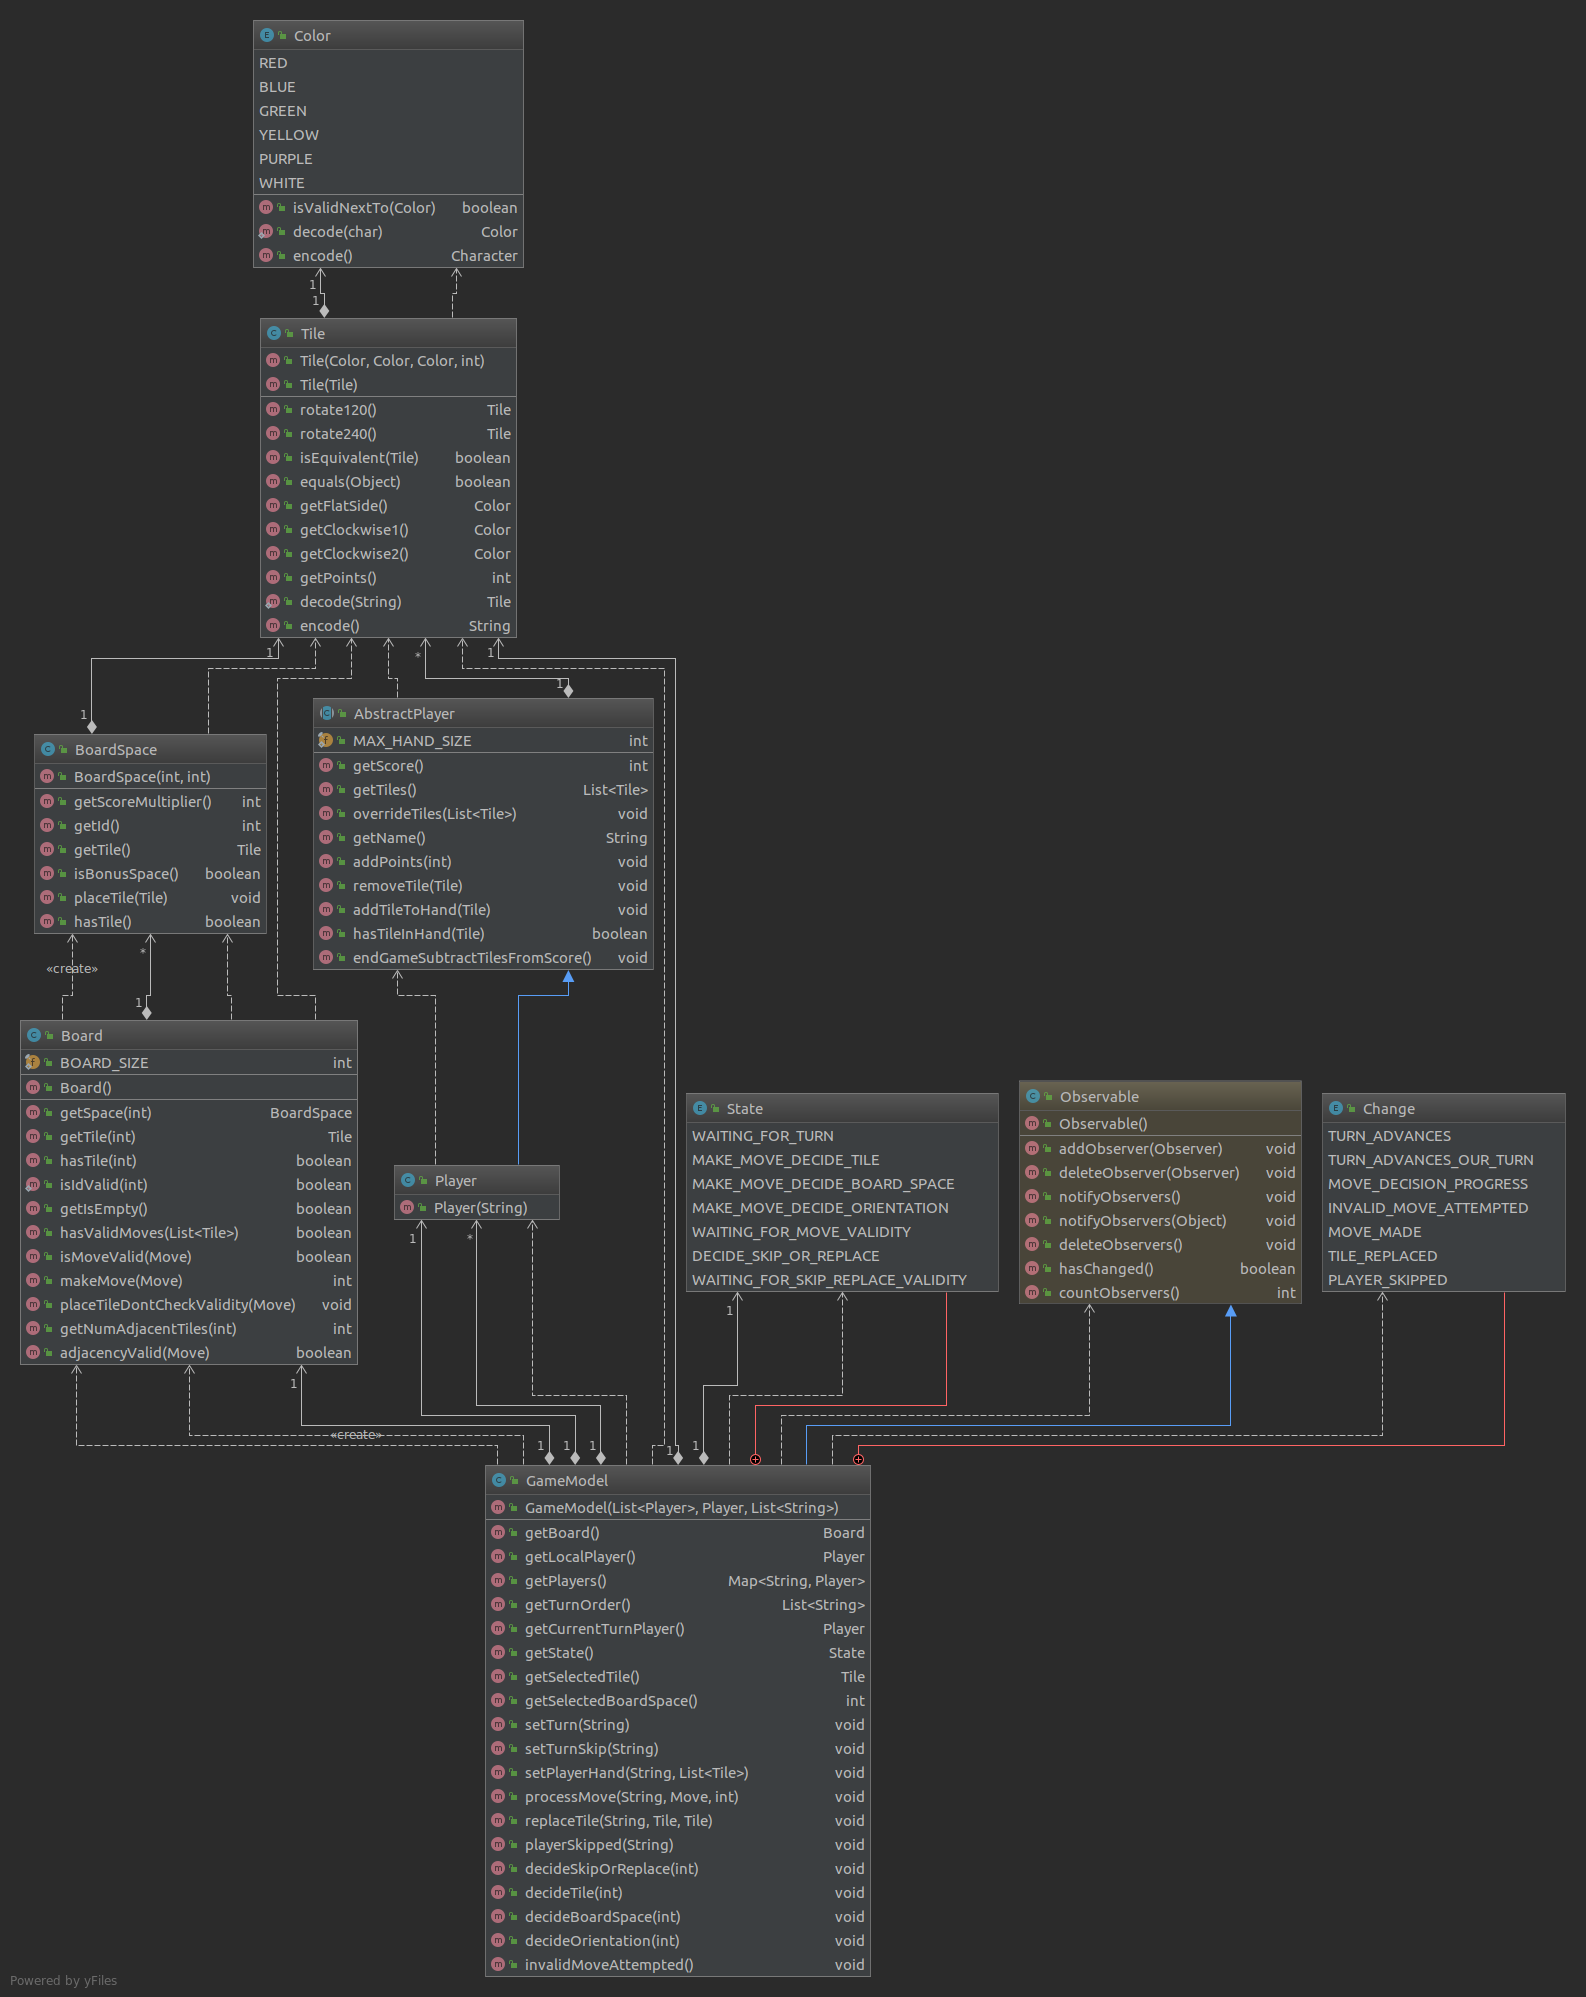
\includegraphics[width=\textwidth]{GameModel.png}
            \caption{Class diagram of the GameModel and the other self-defined classes it contains.}
            \label{fig:modelDiagram}
        \end{center}
    \end{figure}


\end{document}
